\documentclass[11pt,a4paper]{article}
\usepackage[utf8]{inputenc}
\usepackage{amsmath}
\usepackage{amsfonts}
\usepackage{amssymb}
\usepackage{graphicx}
\usepackage{soul}
\usepackage{fullpage}
\usepackage{float}
\restylefloat{table}
\usepackage{tabto}
\usepackage{tikz}
\usetikzlibrary{positioning}
\newdimen\nodeDist
\nodeDist=35mm


\begin{document}

\begin{titlepage}
\begin{center}

% Upper part of the page. The '~' is needed because \\
% only works if a paragraph has started.


\textsc{\LARGE Delft University of Technology}\\[1.5cm]

\textsc{\Large IN4010 Practical Assignment 2}\\[0.5cm]

% Title
%\HRule \\[0.4cm]
{ \huge \bfseries Automated Negotiation \\[0.4cm] }

%\HRule \\[1.5cm]

% Author and supervisor
\noindent
\begin{minipage}{0.4\textwidth}
\begin{flushleft} \large
\emph{Group 11:}\\
Hidde \textsc{Coehoorn}\\
Ralf \textsc{Nieuwenhuizen}\\
Jan-Willem \textsc{van Velzen}
\end{flushleft}
\end{minipage}%
\begin{minipage}{0.4\textwidth}
\begin{flushright} \large
\emph{Supervisor:} \\
Reyhan \textsc{Aydogan}
\end{flushright}
\end{minipage}

\vfill

% Bottom of the page
{\large \today}

\end{center}
\end{titlepage}

\newpage


\section{Introduction to assignment}

As part of the TU Delft course IN4010 Artificial Intelligence Techniques completion of a practical assignment on automated negotiation is required. This is the assignment report of group 11, of which the group members are Hidde Coehoorn, Ralf Nieuwenhuizen and Jan-Willem van Velzen.\\

The subject of the assignment is multilateral negotiation taking place in a multi-issue negotiation domain with discrete issues. The challenge is to design and implement a negotiating agent in GENIUS which can guide the negotiation process and help the parties involved with reaching a satisfying agreement. Various scenarios are created to test the agent, ranging in the degree of conflict between parties.\\

\subsection{Domain}
\label{sec:domain}
Each group had to define their own negotiation domain, complete with multiple issues. Our group chose to create the 'Purchasing a Car' domain. This domain has a total of five issues, each with a number of issue values ranging from two to four (see Table \ref{tab:domainissues}).

\begin{table}[H]
\centering
\caption{The domain issues and issue values.}
\label{tab:domainissues}
\begin{tabular}{|c|c|c|c|c|}
\hline
Power (hp) & Capacity & Mileage (km) & Fuel consumption (km/l) & Wheels \\
\hline
less than 200 & 2 & Below 10.000 & 5 & 3 \\
200 or more & 5 & Between 10.000 and 20.000 & 10 & 4 \\
& 7 & Above 20.000 & 15 & 6 \\
& & & 20 & \\ 
\hline
\end{tabular}
\end{table}


In this domain nine preference profiles are created in three sets of three each. Profiles 1, 2 and 3 will negotiate with one another, as will 4,5 and 6 and so on. The first three profiles are negotiating in a collaborative scenario, the second set is a moderate scenario and the last three profiles clash in a competitive scenario. The specific values of the preference profiles can be found in section \ref{sec:attached_preference_profiles}.


\newpage

\section{Agent}
Besides that our agent is one awesome badass, this might not be obvious by the look of his humble output. There are a couple of ingenious details that are worth pointing out.

\subsection{Tactics}
Our agent has a number of Tactics at its disposal to use at any given moment during the negotiation. These Tactics take the current negotiation state into account, and return an Action based on their nature. \\

\noindent The following Tactics are defined:
\begin{enumerate}
\NumTabs{4}
\item RANDOM
	\tab{Offers a random bid above the reservation value.}
\item BESTNASH
	\tab{Offers the best Nash bid according to the OpponentModels.}
\item NOSTALGIAN
	\tab{Offers the bid from the negotiation history with the highest utility. }
\item ASOCIAL
	\tab{Offers the bid that has the highest utility.}
\item HARDTOGET
	\tab{Offers a bid with 0.99 times the utility of the previous bid.}
\item EDGEPUSHER
	\tab{Offers a bid slightly beter than the previous bid.}
\item GIVEIN
	\tab{Offers a bid that is slightly worse compared to the last.}
\item THEFINGER
	\tab{Leaves the negotiation.}
\end{enumerate}

\subsection{Opponent Utility Model}
\label{sec:opponentutilitymodel}
In order to make a prediction about the utilities of the opponent, we keep track of their actions and compile this into usefull information. Every opponent in the negotiation gets their own model.\\

First of all, we keep counters for all the issue-values in the Domain, and measure how often an opponent includes these values in the bids that it offers. These counts are then used to compute the issue weights and issue-value weights. For every issue, the statistical variance in the issue-value counts is calculated. These are then normalised over all issues, while making sure that no issue has a weight of 0. Lastly, the issue-value weights are made equal to the issue-value counts.

\subsection{Opponent Strategy Model}
\label{sec:opponentstrategymodel}
Besides estimating the opponents utility, we can also make a very rough estimation of the opponents tactic. This metric is only used when it's not possible to create a reliable utility model for the opponent. The model does this by taking the opponents bidding history into account, where it records what bids are done by the opponent, but also what the previous bid was that this new bid could be a response to. Every bid that the opponent has done is then compared to two other bids and a distance measure is calculated. The first bid is the previous bid in the negotiation, the other is the previous bid by the opponent. These can be the same, but most likely won't be. If the distance to the first bid is smaller than the distance to the other bid, it is more likely that the opponent's tactic is to alter the previous bid in the negotiation. If not, it is more likely that the opponent is only changing his own bid every round. 

\subsection{Our own strategies}
\label{sec:strategy}
Apart from the way our agent analyzes its opponents, there is a strategy for its bidding routine as well. We will describe this from the beginning. Furthermore, we would like to state that our agent differentiates between long and short negotiations, because it takes a different strategy for each of them. The critical value is currently set at 20 rounds. All of the described strategies can be seen in figure~\ref{fig:decisiontree}

\begin{figure}[h]
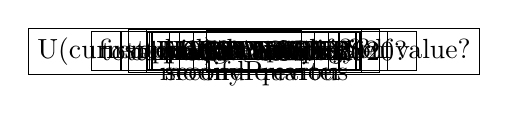
\begin{tikzpicture}[
    node/.style={%
      draw,
      rectangle,
    },
  ]

    \node [node] (A) {U(current bid) $>$ reservation value?};
    \path (A) ++(-135:\nodeDist) node [node] (B) {accept};
    \path (A) ++(-90:\nodeDist) node [node] (C) {current round $>$ 20?};
    \path (C) ++(-135:\nodeDist*1.5) node [node] (D) {opponent strategy?};
    \path (C) ++(-45:\nodeDist) node [node] (E) {total nr. of rounds $>$ 20?};
    \path (D) ++(-135:\nodeDist) node [node] (F) {BESTNASH};
    \path (D) ++(-90:\nodeDist) node [node] (G) {EDGEPUSHER};
    \path (D) ++(-45:\nodeDist) node [node] (H) {BESTNASH};
    \path (E) ++(-45:\nodeDist) node [node] (I) {RANDOM};
    \path (E) ++(-90:\nodeDist) node [node] (J) {enough accepts?};
    \path (J) ++(-135:\nodeDist) node [node] (K) {EDGEPUSHER};
    \path (J) ++(-45:\nodeDist) node [node] (L) {what time is it?};
    \path (L) ++(-135:\nodeDist) node [node] (M) {HARDTOGET};
    \path (L) ++(-90:\nodeDist) node [node] (N) {NOSTALGIAN};
    \path (L) ++(-45:\nodeDist) node [node] (O) {GIVEIN};

    \draw (A) -- (B) node [left,pos=0.5] {yes}(A);
    \draw (A) -- (C) node [right,pos=0.5] {no}(A);
    \draw (C) -- (D) node [left,pos=0.5] {yes}(A);
    \draw (C) -- (E) node [right,pos=0.5] {no}(A);
    \draw (D) -- (F) node [left,pos=0.5] {unknown}(A);
    \draw (D) -- (G) node [below,pos=0.5] {modifyPrevious}(A);
    \draw (D) -- (H) node [right,pos=0.5] {modifySelf}(A);
    \draw (E) -- (I) node [right,pos=0.5] {yes}(A);
    \draw (E) -- (J) node [left,pos=0.5] {no}(A);
    \draw (J) -- (K) node [left,pos=0.5] {yes}(A);
    \draw (J) -- (L) node [right,pos=0.5] {no}(A);
    \draw (L) -- (M) node [left,pos=0.5] {first quarter}(A);
    \draw (L) -- (N) node [below,pos=0.5] {second quarter}(A);
    \draw (L) -- (O) node [right,pos=0.5] {last half}(A);
\end{tikzpicture}
\caption{The decision tree of the agent's strategy} \label{fig:decisiontree}
\end{figure}

%[,rectangle, s sep=35pt,
%  [,edge label={node[Below]{option1}}
%    [,edge label={node[Below]{a longer text goes here}}
%    ]
%    [,edge label={node[Above]{text}}
%    ]
%  ]
%  [,edge label={node[Above]{option2}}
%    [,edge label={node[Below]{a longer text goes here}}
%    ]
%    [,edge label={node[Above]{text}}
%    ]
%  ]
%]



\subsubsection{The first bid}
For the first bid, we really like to make a statement, so we choose the ASOCIAL tactic, which means we offer the best bid for ourselves.

\subsubsection{Accepting offers}
Apart from several accepting stages in the tactics that will be explained in the next sections, there are certain offers that will be accepted at any time. One possibility is an offer with a utility that is higher than the reservation value. This will always be accepted. This may sound weird, but the reservation value starts off at 0.95, which is not bad at all! This reservation value can be lowered in the final stage (see section~\ref{sec:finalstage}), or when the majority of other parties seems to accept an offer. In this last case, the reservation value is multiplied by 0.6, so the offer might be accepted then.

\subsubsection{Long negotiation}
In a long negation (i.e. there are more than 20 rounds in total), we have the possibility to build a trustworthy opponent model.
\\\\
As long as we do not have this model yet (20 rounds have not passed yet) we will apply the RANDOM tactic, which means we will do a random offer above our reservation value. The opponent will either accept, which is fine, or offer according to its own strategy, which is also fine, because that means we can determine its preferences.
\\\\
After 20 rounds we will have a trustworthy model, so we will act according to that. Right now, the most important part of this, is when the opponent is believed to offer bids depending on our own bids. When this is the case, we will apply the EDGEPUSHER tactic, which tries a slightly better offer for us each round, to see whether the opponent might modify that and make a better offer for us to accept. If the opponent is likely to modify his own bids or if the strategy is unknown, we apply the BESTNASH tactic. This picks the best offer from a list of bids sorted on their calculated Nash product, determined by using the opponent models. This bid may change every round due to other offers the opponents might make.

\subsubsection{Short negotiation}
In a short negotiation (i.e. there are less than 20 rounds in total), we will never have a trustworthy opponent model. We will now apply a tactic based on the time that is left for this negotiation.
\\\\
In the first quarter of the negotiation, we will apply the HARDTOGET tactic, which means we will offer a bid with a utility around 0.99 times the utility of our last offer.
\\\\
In the second quarter of the negotiation, we will apply the NOSTALGIAN tactic, which means we will stick to the best bid that has been done during the entire negotiation.
\\\\
Finally, in the last half of the negotiation, we will apply the GIVEIN tactic, which is very descriptive in itself. We will give in a bit. Each next offer is around the utility of $reservation value * utility of last offer$, so each offer is more like to be accepted by the opponents.
\\\\
As a final remark to the short negotiations, it has to be said that if the majority of people accepted an offer, we will at any time apply the EDGEPUSHER tactic.

\subsubsection{The final stage}
\label{sec:finalstage}
When the time is running out, we believe that making a bad agreement is always better than making no agreement. Therefore, we will accept any offer when the negotiation is over 95\% of time.
\\\\
To prevent that this final accepted offer is not the worst for us, starting from 85\% of time, we are lowering our reservation value. Whereas this is 0.95 before this stage, it is now linearly lowered down to 0.5 at 95\% of time. Do you recall that we accept any offer above our reservation value? Well, this works! So most likely, an accepting offer is made before we reach 95\% of time, which will most likely be quite good.

\subsection{How to read this in the source code}
Even though the source code is well documented, it may be hard to figure out where to start, so here we will provide an explanation of its structure.

\subsubsection{The negotiation agent / Group11.java}
This is the main class of our agent. All the other classes are used from here, and this class is used to start our agent in GENIUS. There are several methods in this class that we will address. Every other method is provided with JavaDoc as well, so it should be clear from the source code what each method does.

\begin{itemize}
\NumTabs{6}
\item \textbf{chooseAction}
	\tab{This method is called by GENIUS each round, and it should return the action this agent is going to perform, which can be an Accept, an Offer, or an EndNegotiation. What this method does for us is checking whether the reservation value should be changed, checking whether the previous offer is acceptable, based on those parameters, and otherwise choose the tactic to apply, based on the strategy described in section~\ref{sec:strategy}.}
\item \textbf{getActionForTactic}
	\tab{This method is called from the chooseAction method, and basically it just defines the different tactics.}
\item \textbf{receiveMessage}
	\tab{This method is called by GENIUS every time \textit{any} agent performs an action, including this agent. Here we create an opponentUtilityModel for each opponent, and fill it with the offers they make and the offers they accept.}
\item \textbf{getNashUtilityProduct}
	\tab{Based on a list of opponent models, this function determines the Nash product for a certain bid.}
\end{itemize}

\subsubsection{The opponent model / OpponentUtilityModel.java}
This class is instantiated for each opponent of our agent, and it contains the counters for each issue in the domain. It also uses the OpponentBidHistory and the Statistics classes. We will not describe any method of this class in detail, we will just say it implements the models described in sections~\ref{sec:opponentutilitymodel}~and~\ref{sec:opponentstrategymodel}.

\begin{figure}[h]
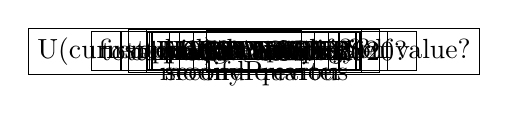
\begin{tikzpicture}[
    node/.style={%
      draw,
      rectangle,
    },
  ]

    \node [node] (A) {U(current bid) $>$ reservation value?};
    \path (A) ++(-135:\nodeDist) node [node] (B) {accept};
    \path (A) ++(-90:\nodeDist) node [node] (C) {current round $>$ 20?};
    \path (C) ++(-135:\nodeDist*1.5) node [node] (D) {opponent strategy?};
    \path (C) ++(-45:\nodeDist) node [node] (E) {total nr. of rounds $>$ 20?};
    \path (D) ++(-135:\nodeDist) node [node] (F) {BESTNASH};
    \path (D) ++(-90:\nodeDist) node [node] (G) {EDGEPUSHER};
    \path (D) ++(-45:\nodeDist) node [node] (H) {BESTNASH};
    \path (E) ++(-45:\nodeDist) node [node] (I) {RANDOM};
    \path (E) ++(-90:\nodeDist) node [node] (J) {enough accepts?};
    \path (J) ++(-135:\nodeDist) node [node] (K) {EDGEPUSHER};
    \path (J) ++(-45:\nodeDist) node [node] (L) {what time is it?};
    \path (L) ++(-135:\nodeDist) node [node] (M) {HARDTOGET};
    \path (L) ++(-90:\nodeDist) node [node] (N) {NOSTALGIAN};
    \path (L) ++(-45:\nodeDist) node [node] (O) {GIVEIN};

    \draw (A) -- (B) node [left,pos=0.5] {yes}(A);
    \draw (A) -- (C) node [right,pos=0.5] {no}(A);
    \draw (C) -- (D) node [left,pos=0.5] {yes}(A);
    \draw (C) -- (E) node [right,pos=0.5] {no}(A);
    \draw (D) -- (F) node [left,pos=0.5] {unknown}(A);
    \draw (D) -- (G) node [below,pos=0.5] {modifyPrevious}(A);
    \draw (D) -- (H) node [right,pos=0.5] {modifySelf}(A);
    \draw (E) -- (I) node [right,pos=0.5] {yes}(A);
    \draw (E) -- (J) node [left,pos=0.5] {no}(A);
    \draw (J) -- (K) node [left,pos=0.5] {yes}(A);
    \draw (J) -- (L) node [right,pos=0.5] {no}(A);
    \draw (L) -- (M) node [left,pos=0.5] {first quarter}(A);
    \draw (L) -- (N) node [below,pos=0.5] {second quarter}(A);
    \draw (L) -- (O) node [right,pos=0.5] {last half}(A);
\end{tikzpicture}
\caption{The decision tree of the agent's strategy} \label{fig:decisiontree}
\end{figure}

%[,rectangle, s sep=35pt,
%  [,edge label={node[Below]{option1}}
%    [,edge label={node[Below]{a longer text goes here}}
%    ]
%    [,edge label={node[Above]{text}}
%    ]
%  ]
%  [,edge label={node[Above]{option2}}
%    [,edge label={node[Below]{a longer text goes here}}
%    ]
%    [,edge label={node[Above]{text}}
%    ]
%  ]
%]



\section{Tests we performed}
For the testing of our agent we actually employed an agile development technique. This allowed us to get fast results, and use them right away to implement changes.
\\\\
The real testing was done in the domain described in paragraph~\ref{sec:domain}. Our test case consisted of three parts for each run. We started the collaborative scenario (profiles 1, 2, and 3), the moderate scenario (profiles 4, 5, and 6), and the competitive scenario (profiles 7, 8, and 9), and compared the results to each previous run.
\\
Values from the output we considered were:
\begin{itemize}
\item Whether the graph looked like we expected;
\item Whether or not there was an agreement;
\item How soon the agreement was made;
\item How far the agreement product was from the nash line;
\item Distance to pareto;
\item Distance to Nash (which appeared to be different from the difference between the product and the nash line).
\end{itemize}

When this result was to our liking (i.e. when the solution was still pareto and the distance was closer to Nash), we used to previously implemented change, and went on to the next improvement. When it was not to our liking, or when there was an error, we tried to correct it, or we reviewed our thoughts about the usefulness of this feature.
\\\\
In our agent, there are multiple values and thresholds that we can adjust when competing with a different negotiation agent. For example, the amount of rounds that is needed for us to build a reliable Opponent Model. In the tests that we did, there was never much difference when we changed these values, but this is because we were only able to test against ourselves. Secondly, our agent is based on a utility model of the opponent, and not based on the bids themselves. This makes it hard to get varying results, when all we can test against is ourselves. 

\subsection{Estimated preference profiles}

After dialing in our agent, we decided to compare the actual preference profiles with the ones we estimate for an opponent.
The estimated values we obtained can be found in section \ref{sec:attached_estimated_preference_profiles}. Note: we were unable to create reliable preference profiles for profile 1, 2, 3 and 4, because these accepted the offers before the 20 round mark. Also,the estimated profile 5 and 6 are based on only 20 rounds, since (because of their nature) they are not that competitive and reach an agreement relatively quickly. The remaining profiles 7, 8 and 9 are based on 150 rounds of data.
\\\\
What can be seen if these results are compared with our actual preference profiles, is that they do give an indication what the main preference of the agent is, but for the other preferences the estimation can be very off. This result can be explained by the agent only negotiation with a clone of itself, which both do not bid based on the issues, but based on the utilities. We are sure that, when faced with a different opponent that adjusts its issues, the estimations will be more accurate.

\section{Conclusions}

We quite enjoyed discussing about the different actions our agent might take in different situations. As this was very close to real life, we could just think ``what would I do?'', and discuss about that. It all seemed very intuitive to us. It was also fun to invent and implement our own smart analyzing tools, like the OpponentUtilityModel. This way it really feels like we are making a smart person to analyze the opponent and do the negotiation for us.
\\\\
In order to be able to support human negotiations in the real world, our agent would need to understand some sort of input, and provide even more extensive output, to let the human know how he is reasoning. Apart from that, we think this agent is already quite versatile, as it can deal with various situations and always seems to find its way. The testing part may prove otherwise though, we are curious about that.
\\\\
To really take over the human negotiation, it would be nice to have some form of computer vision as well, to be able to recognize facial expressions in the opponents, and use that to determine their mood and their feelings regarding an offer. Apart from this, it should probably also be able to handle multiple offers at the same time, as human negotiation is unfortunately less structured than agent negotiation.

\newpage

\section*{Report requirements and checklist}

10 A4 pages may be enough, 15 A4 pages maximum\\
The report should include:\\
\begin{itemize}
\item \st{the group number}
\item an introduction to the assignment
\item a high-level description of the agent and its structure, including the main Java methods (mention
these explicitly!) used in the negotiating agent that have been implemented in the source code
\item an explanation of the negotiation strategy, decision function for accepting offers, any important
preparatory steps, and heuristics that the agent uses to decide what to do next, including the factors
that have been selected and their combination into these functions
\item a section documenting the tests you performed to improve the negotiation strength of your agent.
You must include scores of various tests over multiple sessions that you performed while testing
your agent. Describe how you set up the testing situation and how you used the results to modify
your agent
\item a conclusion in which you summarize your experience as a team with regards to building the
negotiating agent and discuss what extensions are required to use your agent in real-life negotiations
to support (or even take over) negotiations performed by humans.
\end{itemize}

\textbf{The final analysis report should involve an elaborate analysis of your agent's performance from different perspectives (e.g. individual utility gained, social welfare - the sum of utilities of all agents, optimality of the outcome, fairness etc.). NU NOG NIET NODIG}

\end{document}
